\headletter{T}
his Chapter reports the current status of a research that is still ongoing. Starting from the Semantic Web of Things Ontology presented in the previous Chapter, we hereby proceed studying how it would be possible to apply this semantic approach to address real problems.

To do so, Section~\ref{ssec:61_rw} provides some references to the origins of this research and to other relevant works on the subject. Section~\ref{ssec:cocktail}, then, develops a practical implementation for the ontological work available in Section~\ref{sec:swot_ontology}. The \textit{Cocktail} framework is presented, described in detail and realized. Eventually, in Section~\ref{ssec:app_examples} various examples inspired by real world needs are given. Once analyzed, we show our possible solutions with increasing complexity, by exploiting Cocktail and the Semantic Web of Things ontology alongside with other relevant methodologies.

The Chapter takes inspiration from the works published and submitted during the PhD\footnote{~\faCopyright~2019 IEEE~~Reprinted, with permission, from Antoniazzi, F. \& Viola, F. (2019) Building the semantic web
of things through a dynamic ontology. IEEE Internet of Things Journal, early access}.

\section{Related Works}
\label{ssec:61_rw}
Agent-oriented programming idea was originally introduced by Yoav~Shoham in 1993~\cite{shoham1993agent}. Within his exceptional work an extended view is proposed over object-oriented programming: agent-oriented programming interprets systems as a continuous collaboration and competition of computational entities. Such entities, i.e. the agents, are modeled as the result of complex mutual influences of \textit{beliefs}, \textit{decisions}, \textit{capabilities} and \textit{obligations}. Along with this work, similar theories can also be listed, like the Belief-Desire-Intention (BDI) by Georgeff et al.~\cite{georgeff1998belief}.

The belief, first of all, is related with the knowledge of the agent's relevant surrounding environment and entities. In literature this facet was later on intended as the context, and was declined in works focusing on the so called context-aware computing \cite{schilit1994context, dourish2001seeking}. Abowd et al. suggested in~\cite{abowd1999towards} a definition of context that is still up-to-date:
\begin{quote}
Context is any information that can be used to characterize the situation of an entity. An entity is a person, place, or object that is
considered relevant to the interaction between a user and an application, including the user and applications themselves.
\end{quote}
From this definition on, a plethora of works started to explore the subject. Just to name a few, Kofod-Petersen et al.~\cite{kofod2005using} used activity theory to connect contexts to task identification; Sezer et al.~\cite{sezer2018context} surveyed the relationships between context awareness, Internet of Things and Big Data. Baldauf et al.~\cite{baldauf2007survey}, among many others \cite{gu2004ontology, broens2004context, alirezaie2017ontology, cabrera20193lconont}, outlined the relevance of Semantic Web in this discussion introducing ontologies to realize applications.  

Decisions and capabilities, secondly, define the agent's potential influence over the context. The set of capabilities, on one hand, should contain description of what agents can do, regardless their local status. This is the reason why, recently, the concept of capability was declined in works on device discovery mechanisms both in academy (e.g., \cite{ccori2016device, ashraf2016device}) and in industry (e.g. \cite{zhou2017server}, and the already cited work within W3C WoT Working and Interest groups). 

Decisions, on the other hand, would outline the connection between the current context and the most relevant and applicable capability available, to maximize compliance with obligations. To achieve these results, indeed, current research leverages various Artificial Intelligence (AI) techniques that span from classic AI to machine learning \cite{ding2013intelligent, wanigasekara2016bandit}, as well as, in our case, to the usage of semantic information \cite{kovacs2016standards, ganzha2017semantic}.

Lastly, obligations: they are the constraints that agents must respect. Usually, the first idea of ``obligation'' presented to students is given by I.~Asimov's Three Laws of Robotics included in the well-known novel \textit{I,~Robot}. Although they have been source of prolific discussion (e.g., \cite{murphy2009beyond}) over the last decades because of their visionary relevance, it is clear that with the advent of IoT systems the concept of obligation was slightly redirected on a different level. Obligations can be related to constrained device environments \cite{bormann2014terminology}, minimize power, maximize security and privacy, and so on \cite{haroon2016constraints}, or related to the application business logic.

Both the works by Shoham and Georgeff were made before the pervasive electronics and connected IoT real revolution. Over the time, the exponential increase in the number of devices reached a bottleneck in system integration and in capability of interoperate \cite{al2015toward, hossain2015towards}. The context awareness, as discussed, would move to a context of contexts, to create systems of systems into an ``Agents of Things'' environment \cite{mzahm2013agents}. Consider also, in this field, the survey by Kotseruba et al. \cite{kotseruba201840}.

The Semantic Web revealed itself to be part of this discussion according to the view summarized in the previous Sections of this Thesis, and in particular our dynamic approach and exploitation of graph knowledge bases. With reference to the BDI model, the SWOT ontology will hereby be our tool to allow intelligent behavior of agents, through SEPA mediated semantics.

\section{SWOT agents framework and Evaluation}
\label{ssec:cocktail}

This Section contains the discussion over the SWOT ontology and its conceptualization into the Cocktail framework. To do so, the first Subsection will describe Cocktail and show how the ontology can be easily employed to build interoperable applications. Afterwards, an overall evaluation of the SWOT ontology will be provided, according to a set of literature metrics.

\subsection{Cocktail framework}
\label{ssec:cocktail_framework}
Once the SWOT ontology is given and both its static and dynamic parts have been addressed, we have the ingredients to setup a Semantic Web of Things environment. As already stated in the previous Sections, in our implementation the SEPA has been adopted to dispatch events and notifications to control the dynamic evolution of the SWTE. On the other hand, the Web Things will use instances of the static subset of the SWOT ontology to declare themselves and to discover their context. In a broader view, starting from here, the SEPA may act as a Semantic Cloud engine for a generalized Semantic Web of Things over the SWOT ontology.

To do so, the SEPA implementation available on Github\footnote{\faGithub~\url{https://github.com/arces-wot/SEPA}} will be used together with the baseline APIs developed for it\footnote{\faGithub~\url{https://github.com/arces-wot/SEPA-python3-APIs} (branch \texttt{dev-0.9.5})}. On top of them the Semantic WoT SEPA APIs are built as a complete framework named \textit{Cocktail}. The Cocktail framework is also freely available on Github\footnote{\faGithub~\url{https://github.com/fr4ncidir/SemanticWoT}} with its documentation and the explanation of the reasons behind its name. 

Cocktail contains high level functions and classes to:
\begin{enumerate}
    \item Declare the things, assign them a friendly name, an URI, and a thing description resource;
    \item Append to the thing description resource all the interaction patterns needed, i.e., actions, events, properties, with their friendly names, URIs, data as described in Section~\ref{ssec:interaction_patterns};
    \item Define, if needed, new data schemas;
    \item Query the SWTE for things, interaction patterns, and basic discovery mechanisms;
    \item Request the execution of an action, post its output and wait for it if necessary, together with all the needed timestamps;
    \item Throw, and wait for event notifications;
    \item Delete those instances.
\end{enumerate}

All these functions, indeed, share a common point. They perform specific requests to SEPA: either SPARQL Updates, or SPARQL Queries, or SPARQL Subscriptions. Cocktail uses SPARQL Updates to spawn new things, actions, events, properties and data schemas and their internal relationships; in addition to that, they are needed also to inject in the graph new action or event instances and output data. Those triples, once inserted in the knowledge base, will be captured by the SEPA subscriptions engine, that will trigger an action execution, or notify that an event has occurred or that an output is available. Eventually clients, humans or Web Things, will be allowed to perform SPARQL Queries looking for all kinds of information in the graph: e.g., we expect standard requests like \textit{``List all Web Things in the SWTE''} along with more complex ones, like \textit{``What interaction patterns give as output mp3 files?''} or \textit{``What Web Things have at least an action which is described through the Pizza Ontology?''} or also \textit{``How can I format my data so that a specific action can use it as input?''}

It is therefore clear that Cocktail is composed by two facets: the SPARQL code, that interacts with triples in the knowledge base; and the thing business logic, that takes care of performing the main tasks of the device, and the communication with SEPA. In our implementation, targeting a proof of concept rather than a full realization of the platform, Python3 has been adopted to address the thing business logic. Indeed, equivalent APIs will be developed for other languages in the future, to be used also in more constrained devices, like the Arduino family and so on. 

It is worth noticing that the SPARQL code remains the same in all those implementations. As already said, it is available in Cocktail repository, to be used within our Python3 setup or to be called directly from others services.

%All the classes in Cocktail offer a method \texttt{post}, with which the semantic description is updated to the SEPA engine on top of the knowledge base. Similarly, they also have a \texttt{delete} method, which is a way to remove the description from the graph storage. Additionally, there is another common method, the \texttt{discover}, that represents the core of discoverability in the SWTE. The default \texttt{discover} methods available in Cocktail classes refer to the basic mechanisms that mainly look in the knowledge base for all Things, all Actions, and so on. For the future, we consider that various semantic discovery queries will be developed, basing on the ontology presented in this paper and on all its possible interactions with other ontologies.

%Together with posting and discovering things, one of the most important aspects of Semantic WoT that Cocktail deals with is the request-response protocol we described in Section \ref{sec:interactions} when Actions and Events interact.

%For this reason, in the Cocktail framework the Actions have some methods that are bound to subscriptions. One of them, for instance, is the method that requests an Action performance, giving all the needed information on parameters. The WebThing, being notified by SEPA of the request, triggers accordingly its task to be performed, which is triggered when the SEPA notifies the request, can be given as a python script, and we can enable or disable its execution. The requesting entity, then, subscribes 

%Concerning Events, Cocktail embeds the SPARQL update with which Events can notify the occurrence of something. Third parties, then, need to be able to subscribe to those notifications, and get the output (if any).

\subsection{Cocktail: in-use analysis}
\label{ssec:cocktail_eval}
Cocktail's collection of SPARQL updates, queries and subscriptions on top of SEPA proves that a Semantic WoT implementation is achievable in an overall limited amount of lines of code.

Nevertheless, an evaluation is required, both of the framework's usability and of the ontology itself. Notice that an evaluation of the SEPA and its processing units is not within this paper's scope.

% \begin{lstlisting}[caption={Smart discovery for Web Things with an Action acting on temperature and requiring a $\psi$-formatted input}, label=listing:smart_discovery1, mathescape]
% SELECT ?thing ?action 
% WHERE {
%   ?thing rdf:type swot:Thing, sosa:Actuator;
%     sosa:actsOnProperty ns:Temperature;
%     swot:hasThingDescription/swot:hasAction
%       ?action .
%   ?action swot:hasInputDataSchema <$\psi$_uri>
% }
% \end{lstlisting}

% \begin{lstlisting}[caption={Smart discovery for Web Things that are \texttt{ns:Temperature} sensors triggering Events with $\lambda$-formatted output}, label=listing:smart_discovery2, mathescape]
% SELECT ?thing ?event 
% WHERE { 
%   ?thing  rdf:type swot:Thing, sosa:Sensor;
%     sosa:observes ns:Temperature;
%     swot:hasThingDescription/swot:hasEvent 
%       ?event.
%   ?event swot:hasOutputDataSchema <$\lambda$_uri> 
% }
% \end{lstlisting}

Let's start by analyzing the usage of the framework. To do so, the following small SWTE composed by 3 semantic Web Things (depicted in Fig.~\ref{fig:swte}) and a few additional triples has been developed:
\begin{description}
    \item[\texttt{ns:Thermostat}] is a smart thermostat also declared as a \texttt{sosa:Sensor} observing the special resource \texttt{ns:Temperature} (2 additional triples). This smart Web Thing has an action called \textit{ThresholdAction}, and an event called \textit{TemperatureEvent}. By calling the \textit{ThresholdAction}, the user can define $T_{low}$ and $T_{high}$, and therefore setup his/her desired temperature interval. The thermostat performs also a smart discovery: it looks for Web Things acting on \texttt{ns:Temperature}, and providing an action that requires some input formatted with a specific data schema $\psi$. The SPARQL code used for discovery is available in Listing \ref{listing:smart_discovery1}. If there are available actions of this kind, and the temperature $t\not\in [T_{low},T_{high}]$, the thermostat triggers \textit{ThresholdAction}. Every 5 seconds, also, the thermostat throws a \textit{TemperatureEvent} with the current temperature value (data schema $\lambda$).
    \item[\texttt{ns:HotCold}] is a smart air conditioner and heater. It is also typed as \texttt{sosa:Actuator} acting on resource \texttt{ns:Temperature} (2 additional triples). It has an action that can be triggered with input formatted according to dataschema $\psi$. The device performs a different smart discovery, available in Listing~\ref{listing:smart_discovery2}, searching for \texttt{ns:Temperature} sensors and subscribing to their temperature-change event formatted as $\lambda$ data schema. 
        \item[\texttt{ns:Clock}] is a smart clock with an action that, when requested, replies with the current timestamp (data schema $\xi$), and an action that replies with the current temperature (data schema $\lambda$). Also, \texttt{ns:Clock} is a \texttt{sosa:Sensor} observing \texttt{ns:Temperature} (2 additional triples). It's worth saying that this is a dummy device that proves the effectiveness of smart discoveries: Listing~\ref{listing:smart_discovery1} discovery will not match with \texttt{ns:Clock}, because it is not a \texttt{sosa:Actuator}, and Listing~\ref{listing:smart_discovery2} because there is no corresponding Event.
    
    %\todo{When you write the words "Action" or "DataSchema" you should use capital letters only if you really want to recall the ontology class. In that case, use \texttt{\textbackslash texttt}, it's better. Otherwise, don't use capital letters, as in the speech \textit{normal} words do not require them. -- Fabio}
    
    \item[Other triples] are related to the resource \texttt{ns:Temperature} and to the data schemas. In order to allow the more complex discovery methods previously cited, two \texttt{rdf:type} references are added to the temperature resource using the SOSA ontology,\\ \texttt{sosa:ActuatableProperty} and \texttt{sosa:ObservableProperty} (2 additional triples).
\end{description}

\begin{lstlisting}[caption={Smart discovery for Web Things with an Action acting on temperature and requiring a $\psi$-formatted input}, label=listing:smart_discovery1, mathescape]
SELECT ?thing ?action WHERE {
  ?thing rdf:type swot:Thing, sosa:Actuator;
    sosa:actsOnProperty ns:Temperature;
    swot:hasThingDescription/swot:hasAction ?action .
  ?action swot:hasInputDataSchema <$\psi$_uri>
}
\end{lstlisting}

\begin{lstlisting}[caption={Smart discovery for Web Things that are \texttt{ns:Temperature} sensors triggering Events with $\lambda$-formatted output}, label=listing:smart_discovery2, mathescape]
SELECT ?thing ?event WHERE { 
  ?thing  rdf:type swot:Thing, sosa:Sensor;
    sosa:observes ns:Temperature;
    swot:hasThingDescription/swot:hasEvent ?event.
  ?event swot:hasOutputDataSchema <$\lambda$_uri> 
}
\end{lstlisting}

\begin{figure}[h!]
    \centering
    \includegraphics[scale=0.7]{swte3.png}
    \caption{An example of Semantic Web Thing Environment}
    \label{fig:swte}
\end{figure}

As stated in Section~\ref{ssec:dataschema_fieldschema}, all the dataschemas $\psi, \lambda, \xi$ are considered to be already available in the SWTE. Given that, if we imagine that temperature is $t=3^{\circ}C$ and $T_{low}=18^{\circ}C$, what happens in this environment is that:
\begin{itemize}
    \item if the thermostat is declared first it will only notify the temperature event until the smart discovery is becomes effective. Once \texttt{ns:HotCold} is available, the thermostat is notified that an action formatted as requested is now present in the SWTE. The action is therefore immediately triggered, and will continue until a temperature event is notified so that $T_{low} \le t \le T_{high}$;
    \item if \texttt{ns:HotCold} is declared first, it will just start waiting normally for its action to be triggered. No temperature event from sensors is available, as \texttt{ns:Clock} generates temperature through an Action. Once, finally, the thermostat is available the Action is triggered upon its request and the temperature starts rising, until it reaches a level between the thresholds.
\end{itemize}
%\todo{Again, consider whether you should use Action, \texttt{Action} or action. I won't highlight all the occurrences :-) -- Fabio}

As it can be seen, Cocktail on its own is enough to build an environment in which semantic Web Things are totally independent, and basic environmental discoveries are available. \textit{Cocktail allowed to concentrate on the basic mechanisms of the SWTE}.

Cocktail alone, however, would have been insufficient to help the thermostat decide the best action to trigger. To make the decision, if the action in \texttt{ns:HotCold} or in \texttt{ns:Clock}, we need to introduce the 8 SOSA-related triples. Those additional triples allowed us to identify the Web Thing needed, the action to be requested and the events to which we have to subscribe. 

%\todo{Note that in the document you name devices both \textit{Web Things} and \textit{WebThings}. We should be consistent throughout the whole paper. -- Fabio}

This result, in particular, proves that our ontology is easily extensible, and that even a small addition to it can lead to interesting autonomous behaviours, by expanding context awareness.

% \todo{This sentence is a bit foggy. When you refer to \textit{interesting results} you should probably mention an example. -- Fabio}

The code realizing the SWTE is available in Cocktail's Github repository, and shows that the realization of the software modules is rather simple and based on a schema that can be summarized as following:

\begin{enumerate}
    \item Identification and description of interaction patterns;
    \item Posting to the SWTE the triples;
    \item Definition of actions' and events' behaviour;
    \item Device loop: business logic, and events' throwing;
    \item \textit{Optional} small Web server dedicated to JSON-LD thing description.
\end{enumerate}

%\fabio{\noindent Important related work:
%\begin{itemize}
    %\item 
%    \item \href{http://www.jsm.or.jp/ejam/Vol.8No.2/AA/AA117/AA117.pdf}{questo}
%    \item \href{https://pdfs.semanticscholar.org/8897/83092fa5ea6201339546a85c7d0b7483902b.pdf}{quest'altro}
%    \item \href{https://www.w3.org/community/owled/files/2016/11/OWLED-ORE-2016_paper_10.pdf}{quest'altro ancora}
%\end{itemize}}

\subsection{Evaluation}
\label{ssec:evaluation}
The task of evaluating an ontology is rather complex due to the fact that it has to be performed as a balance between \textit{expressiveness} and \textit{effective usage}. Although the ontology may address various abstraction levels, the target applications must be taken into account in order to distinguish pros and cons. Philosophical ontologies will be mostly evaluated by their expressiveness, while the engineered ones will need also a contact with real applications.

In this work, furthermore, the target is an even different concept, which is in fact a quite new situation in the panorama: the ontology has been defined as \textit{dynamic} to highlight the fact that it is built up of a descriptive and static part, and of a context-evolutionary part. While proceeding with an empirical evaluation of the work presented in this paper this factor, that has strong relevance in the realization of the whole application, will be taken into account.

Fern\'andez et al.~\cite{fernandez2009what} defined a set of 12 metrics to measure the quality of an ontology. In the current paper those metrics are partially adopted and partially re-arranged to be reasonably applied to the work. In fact, the authors believe that in this specific case, due to the small dimension of this SWOT ontology, not every metric among the ones suggested in origin would be completely appropriate. Keeping this in mind, the evaluation is hereby reported: 
\begin{itemize}
    \item \textbf{Number of classes}: the number of classes in the SWOT ontology. The overall value, for the ontology, is 14: among these, 10 are used for the static SWTE description, and the remaining 4 have a dynamic role;
    \item \textbf{Number of properties}: number of (datatype or object) properties in the ontology. The datatype properties are overall 9, 4 of which allow the static description, and 5 the dynamic one. The object properties, instead, are 9 static, 7 dynamic and 4 belonging to both the sets, 20 in total. Eventually, 20 more (inverse) properties can be added. Being redundant elements, they will not be considered from now on.
    
    %\todo{Remember, we should use capital letters when really needed\dots Probably \textit{object} and \textit{datatype} could be expressed with lowercase letters. -- Fabio}
    
    \item \textbf{Number of individuals}: number of individuals defined in the presented ontology. At present, the SWOT ontology does not include any individuals: however, as it has been already said, \texttt{swot:DataSchema} and the \texttt{swot:FieldSchema} instances are a kind of entity that may be considered similar to the concept of individual, since they should be available in the SWTE before the setup of things, and in general they should not be removed.
\end{itemize}

Those first three points have a considerable impact on the overall composition of a Cocktail-based SWTE because their values affect the complexity of the needed SPARQL enquiries. Being the ontology composition almost equally bipartite, with 27 entries belonging to the static description and 20 belonging to the dynamic evolution, in fact the SPARQL obtained for the complete Cocktail setup appears to be unexpectedly simple. 

Another metric that can help understanding the SWOT ontology capabilities is the number and the sequence of SPARQL interactions (Updates, Queries and Subscriptions) that are required to have a running Cocktail-based SWTE. The metric, similarly, outlines an evaluation of the computational resources necessary for a working SWTE setup, identifying the minimal requirements for a running Web Thing. To give an example, let's consider the same example of Subsection~\ref{ssec:cocktail_eval}, considering Web Things \textit{as is}, out of the general application logic:

%\todo{Advice: when you include a reference (nevermind if it's an internal one or to a bibliography entry) put before a tilde instead of the space character. It is the \textit{unbreakable} space of \LaTeX. In this way you make sure that the number will not be sent to a new line. -- Fabio}

\begin{description}
    \item[\texttt{ns:Thermostat}] requires 6 SPARQL updates to globally post the Web Thing (1), its Action (1) and Event plus its notifications (2). In addition to that, there is also the update for the additional background (1) and, eventually, the external Action request, that is also a SPARQL update. Concerning subscriptions, one permits to be notified of external requests towards the thermostat Action, and one is required for the smart discovery mechanism, as already described in the previous Subsection.
    \item[\texttt{ns:HotCold}] similarly requires 5 updates and 3 subscriptions.
    \item[\texttt{ns:Clock}] requires 4 updates and 2 subscriptions.
\end{description}
In the end, this 3-Web Thing SWTE requires 15 updates (some of which are performed into a loop according to the application logic), and to keep 7 subscriptions opened. Not to mention, moreover, the deletion of resources, once they are no more needed. Most the times (namely, the ones related to the dynamic part of the ontology), the deletion is embedded in the same SPARQL Update that performs triple addition. So, it has been already counted in the previous discussion. The deletion of static resources, on the contrary, is more rare, and we do not count it, as it has to be made on explicit request by the system maintainer.

Indeed, this is an interesting result, even though no graph level security and privacy mechanisms have yet been implemented. For now, by extrapolation from this example, one can notice that the SWOT ontology requires from the device the capability of dealing with $U$ updates, linearly increasing with the number of interaction patterns; and with $S$ subscriptions, whose minimum number increases also linearly on interaction patterns, and whose actual number depends on the application logic involved. In this performance evaluation, eventually, it is important to mention that a great impact is related to subscriptions. They imply, with the SEPA compliant Cocktail implementation, the capability of the device's hardware to keep a WebSocket opened over a long period of time, which is not always possible because of restricted computational or energetic constraints. A complementary solution would be the usage of queries instead, resulting in devices explicit request of the contents of the knowledge base at specific instants. This implementation is not available in Cocktail, but is possible and is scheduled for a future work.

%\todo{The linear dependency is quite easy to notice by reading the text, but a chart could help. -- Fabio -- I would avoid here a chart, as it is an extrapolation and strongly depends on application logic. -- Francesco}

\begin{itemize}
    \item \textbf{Maximum and minimum \textit{Web Thing triple count} $T$}: how many triples are needed to setup a Semantic Web Thing? As it has been already said, this calculation depends on the interaction patterns that the Web Thing has to implement. However, by parsing the SPARQL updates we get a total of
    \begin{equation}
T = 4+9A_{io}+7(A_i+A_o+E_o)+5(A_e+E_e)+13P_v+12P_e+f+C
        \label{eq:webthing_count}
    \end{equation}
    where 4 triples are dedicated to \texttt{swot:Thing} and \texttt{swot:ThingDescription}, 9 to a number $A_{io}$ of input-output Actions, 7 to input, output Actions and output Events, 5 to empty Actions and Events and 13 (or 12) to Properties. To be precise, $P_e$ is the number of Properties that have data formatted as \texttt{swot:ResourceURI} or \texttt{swot:OntologyURI}, and $P_v$ the ones that have data as a literal). A constant $f$ is related to \texttt{swot:forProperty} connections, and $C$ includes connections to third parties ontologies. Notice that $f$ cannot be greater that the number of Actions and Events times the number of Properties.
    
    Given this, concerning the static description of Web Things, it is possible to outline that 4 triples is the absolute minimum reachable for a special Web Thing without Interaction Patterns, and that Properties are the pattern that requires the greatest number of triples, due to the fact that they store also data. 
    
    %\todo{Here you talk about a minimum and a maximum, but then you provide only an equation to get \textit{T}. Even if it is absolutely clear that you obtain the minimum and the maximum by considering respectively 1 device and a maximum number $n$ of devices, I would state it explicitly. Also note that this sentence is quite inspiring to plot some charts\dots -- Fabio}
    
    \item \textbf{Triple count for interactions and $DvS$ ratio}: how many triples are inserted when a new action request is made, or when a new event notification is triggered? Similarly to Equation~\ref{eq:webthing_count}, it is possible to obtain the number of triples required for the dynamic control of event and action instances. Refer to Fig.~\ref{fig:fig5} to observe in each situation what are the requirements. 
    
    Fig.~\ref{fig:fig5} also introduces the \textit{dynamic vs static} ($DvS$) ratio (i.e., the triple count for static description over the triple count for dynamic interaction). $DvS$ depends on the kind of interaction pattern only and is bound to the Web Thing functionality within its context. It is therefore a metric that is obtainable only once its description according to Section~\ref{ssec:interaction_patterns} has been defined by the programmer. $DvS$ ratio can be applied to a real Web Thing with all its setup: the greater the ratio, the higher the Web Thing requirements in term of real-time interactions.
    \item \textbf{Data format influence on triple dimension}; as explained in Section~\ref{ssec:dataschema_fieldschema} the format of data exchange is of great importance. The complexity of the description of any SWoT device, however, does not depend on that of exchanged data, nor on its dimension or type. The possible alternatives have been fully described and exemplified in Tables~\ref{tab:event_instance}~and~\ref{tab:action_instance}, which show that the number of triples exchanged is the same. 
\end{itemize}

\begin{figure*}
    \vspace{10pt}
    \centering
    \includegraphics[width=\textwidth]{Immagine2.png}
    \vspace{10pt}
    \caption{Number of triples for every interaction pattern, and their $DvS$ ratio value maximum and minimum.}
    \label{fig:fig5}
\end{figure*}

%    \item \textbf{Maximum and minimum depth}: respectively the size of the longest and shortest branches in the ontology.
%    \item \textbf{Average depth}: average size of the branches of the given ontology.
%    \item \textbf{Depth variance}: variance of the size of the branches in the SWoT Ontology.
%    \item \textbf{Maximum, minimum and average breadths}: size of the largest/narrowest/average levels of the ontology here presented.
%    \item \textbf{Breadth variance}: variance of the size of the levels in the SWoT Oontology.  

In order to make a more complete evaluation of SWOT ontology, some additional considerations can be made thanks to the usage of online tools like PerfectO\footnote{\faLink~\url{http://perfectsemanticweb.appspot.com/?p=ontologyValidation}} and OOPS!\footnote{\faLink~\url{http://oops.linkeddata.es/}}. By performing a scan of SWOT ontology through the tools listed in those websites, we were able to make relevant enhancements to SWOT ontology.

OOPS! tool, however, provides only a formal check of the \texttt{.owl} file, while a global view is also needed. This kind of evaluation is possible by examining our work through a set of criteria globally accepted by the research community. As an example, the guidelines for submission to the well-known ISWC Conference\footnote{\faLink~\url{http://iswc2018.semanticweb.org/call-for-resources-track-papers/\#}} are very helpful. Most of the suggested points were largely covered in the previous Sections and/or in Tables~\ref{tab:miro1}, \ref{tab:miro2}, \ref{tab:miro3}. What has to be noticed globally is that SWOT ontology addresses a relevant topic of current research that targets a fusion of Semantic Web and IoT and provides tool for a working implementation. Moreover, it is documented and freely available on GitHub, GNU GPL licensed, but, as a work in progress, still not submitted to community registries like LOV.

\section{Next Steps}
\label{ssec:app_examples}
This Section will address the possibilities that Cocktail offers when the Semantic WoT Environment (see SWTE definition in Section \ref{ssec:semantic_web_things}) created is intended to work in collaboration with some AI mechanisms. A general idea has been already given in Section \ref{ssec:cocktail_eval}, although we will here discuss in more detail the opportunities and the setups. 

In addition to what has been introduced in the previous paragraphs, we will also refer to the ideas expressed in some research papers that have been published \cite{antoniazzi2017web, paolini2019fall, paolini2019anchorless} over the time at (or with the collaboration of) ARCES lab. 

While reading this Section please consider that some of the suggestions given are either pending research (as of October 2019), either planned for future studies and implementations. Although not yet complete, they deserve to be mentioned anyway because they participated as a global frame to the creation of this Thesis work.

\subsection{Cocktail example}
Let us now consider the setup described to explain Cocktail available in Fig.~\ref{fig:swte} and fully discussed in Section \ref{ssec:cocktail_eval}. As we said, by the means provided by SEPA our small application was using the SPARQL subscriptions to dynamically discover the environment and to call the right \texttt{swot:Action} at the right time, as well as to stop it when there was no more need. In order to autonomously respond to context variations, in particular, the heating unit needed to be informed of the availability of a thermostat capable of formatting its output in a convenient manner. \textit{Vice versa}, the thermostat needed to be aware of heating units close by (see Listings \ref{listing:smart_discovery1} and \ref{listing:smart_discovery2}).

In our case, additionally, the thermostat had to be aware of the requirements coming from the user in terms of expected temperature in the room. Even though that assumption might appear reasonable here, it is worth mentioning that in general this is not the case. It may not always be possible to have such a \textit{Master WebThing}, which we define here as a device containing all the preferences of the user regarding the politics of context control within his/her own domain. 

An IoT environment built up on a middleware setup is probably the easiest way to create the Master WebThing abstraction: all information passes through the central unit, and therefore can be forwarded to the context master for AI elaboration. Clearly, in this description, Cocktail framework and SEPA together offer this capability providing to the Master WebThing the same abstraction as an ordinary WebThing, including a discovery mechanism that is as flexible as SPARQL, as dynamic as publish-subscribe.

The main limit of the example is the way in which the user preference expression $T_{low} \le t \le T_{high}$ is given. As it is now, we have that the preference is hardcoded in the thermostat business logic. Even if Cocktail allows quite easily to add a new Action that modifies the two thresholds upon user request, this solution implies that every other device implementing this rule should be visited and updated in the same way.
\begin{figure*}
\centering
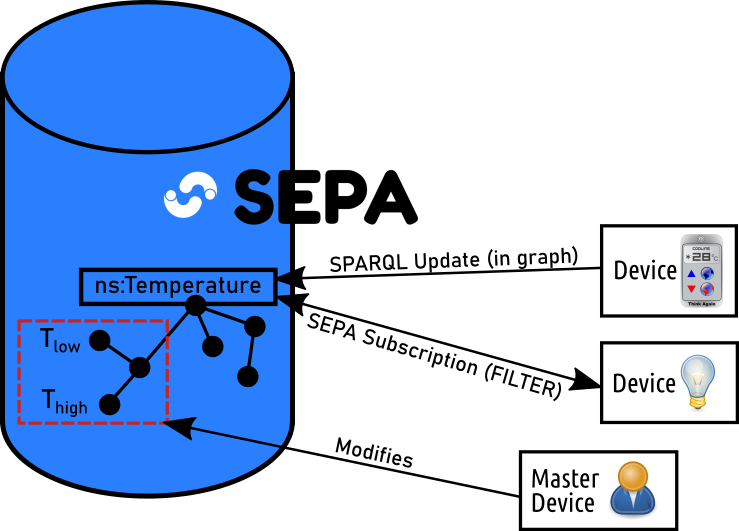
\includegraphics[width=0.7\textwidth]{preferences.png}
\caption{Suggestion for including in Cocktail the concept of \textit{Master Device}, i.e. a device dealing with the user's preferences on context control.}
\label{fig:preferences}
\end{figure*}

A possible alternative, that is currently a preliminary study work still pending implementation is shown in Fig. \ref{fig:preferences} and refers to the Master WebThing concept. First of all, we consider here that the added \texttt{ns:Temperature} resource might be in fact a separate RDF subgraph within SEPA. The temperature graph is required to follow the data schema/field schema concept (see Section \ref{ssec:dataschema_fieldschema}), being formatted in its own specific way. Consequently, any device updating the temperature would make a SPARQL Update similar to the one in Listing \ref{listing:temp_update_subgraph}.

\begin{lstlisting}[caption={SPARQL Update temperature subgraph. Refer to the previous Sections for any unexplained resource. Notice that this is currently (October 2019) an ongoing work and therefore it is not to be considered a final solution.}, label=listing:temp_update_subgraph]
WITH ns:Temperature
DELETE {ns:RoomTemperature swot:hasValue ?v}
INSERT {ns:RoomTemperature swot:hasValue "18.4"}
WHERE {
   ns:RoomTemperature a swot:Data;
   	swot:hasDataSchema ns:MyDoubleDataSchema.
}
\end{lstlisting}

The Master Device on the other hand would take care of the user preferences by modifying the appropriate part of the \texttt{ns:Temperature} subgraph. In our preliminary research we suggest to introduce a new \texttt{swot:Preference} resource type as shown in Listing \ref{listing:pref_update}, defining for the current example the lower and upper boundaries of acceptable temperatures.

Eventually, any device acting due to some temperature specific behaviors would subscribe to that same subgraph, filtering the results according to its own business logic as reported in Listing \ref{listing:pref_subscription}. In this way, each time the temperature falls out of the interval, SEPA triggers the relevant subscriptions based on that resource.

What is still missing in this approach is a complete theory concerning the relationships between different preferences. Are there preferences that are more or less important than others? What would be the effect of this preference ordering in the knowledge base? These are the main future directions for this research.\\
\begin{minipage}{\linewidth}
\begin{lstlisting}[caption={SPARQL Update to temperature preferences. Notice that this is currently (October 2019) an ongoing work and therefore it is not to be considered a final solution.}, label=listing:pref_update]
WITH ns:Temperature
DELETE {
   ns:user_preference ns:lower ?low;
    ns:upper ?high.}
INSERT {
   ns:user_preference ns:lower "18.2";
    ns:upper "28.0".}
WHERE {
   ns:user_preference a swot:Preference.
}
\end{lstlisting}
\end{minipage}
\begin{lstlisting}[caption={Suggested example for SPARQL device FILTER subscription. Notice that this is currently (October 2019) an ongoing work and therefore it is not to be considered a final solution.}, label=listing:pref_subscription]
SELECT ?current
FROM ns:Temperature
WHERE {
   ns:user_preference a swot:Preference;
    ns:lower ?low;
    ns:upper ?high.
   ns:RoomTemperature swot:hasValue ?current.
   FILTER(?current <= ?high)
   FILTER(?current >= ?low)	
}
\end{lstlisting}

Summarizing:
\begin{enumerate}
\item Nothing changes in the PAE interaction paradigm;
\item Target entities like \texttt{ns:Temperature} would be represented as \texttt{swot:Data} within a subgraph;
\item A Master WebThing, described in the same way as other WebThings, would be able to control the user's preferences \texttt{swot:Preference} and modify the target entities accordingly;
\item The devices using the target entities would apply their (autonomous behaviour) business logic based on \texttt{FILTER}ed subscriptions related to \texttt{swot:Preference} instances.
\end{enumerate}

Notice that we have formalized here a \textit{Semantic Belief-Desire-Intention behaviour} \cite{challenger2018development}: the beliefs are the aforementioned subgraphs like \texttt{ns:Temperature}; the desires are the \texttt{swot:Preference} definitions; the intentions are the notification triggers upon \texttt{FILTER}ed subscription.

\subsection{Habitat project example}
The Habitat project acted an essential role in the development of the Semantic Web of Things as intended in this Thesis. Its main contribution, as it will be clear in the next paragraphs, is related to the flexibility in thing description and easy extensibility required to the Habitat IoT-WoT environment. They both had relevant effects in the actual Cocktail implementation.

During the project the author and his colleagues were involved in the creation of an indoor localization IoT environment with the goal of monitoring people with mental impairments. The importance of such systems can be exemplified by a typical use case connected to one of the greatest problems that modern societies are facing, namely the care for people suffering Alzheimer's disease. 

Along with the cognitive decay due to the progression of the disease, it is indeed important to allow the patients to stay safely independent as much as possible so that no stress or technical malfunction could have negative effects on their everyday life. Keeping this in mind, the indoor monitoring provided by Habitat would act as a non invasive control of danger situations, like being close to the stairs, or the patient being almost out of the house without the caregiver supervision.

From a broader point of view indoor monitoring represents a functionality that has various possible applications. Given the versatility of the information retrieved, we have that smartphones apps, social networks, but also police and many others use such information to be more efficient and effective in their jobs of advertising, catching illegal activities and so on.

This is one of the main reasons why the a Semantic approach was preferred within Habitat to control the information flow. The variety of possible usages that can be done of localization information requires a shared and flexible solution for data description. As a consequence, Habitat project outlined on one hand the lower level setup (that are out of the topic of this thesis), i.e. (i) raw data measurements with radio frequency; (ii) fog computing approach retrieving medium-level information, like $(x,y,z)$ coordinates. 

On the other hand, it is important to mention that, on top of the information interoperability, a great achievement was the successful usage of a prototype of Cocktail over SEPA, realizing (iii) information aggregation; (iv) the handling of danger situations by calling the appropriate actuators.

Let us consider point (iv), that was largely addressed in the Sections describing and evaluating Cocktail. Within Habitat we considered two separate possible approaches:
\begin{itemize}
\item If-This-Then-That (IFTTT): the business logic of the IoT environment is realized performing the requests as a set of actions following predetermined conditions. 

\item Rule engines, like Drools \cite{proctor2011drools}: SEPA notifications, in this case, were transformed into events triggering rule evaluation in drools, and resulting eventually in decisions over the environment state.
\end{itemize}

While Habitat project reached its end, there is still the possibility to proceed with some further research in the future. For instance, as the SEPA middleware is common to all these implementations and Cocktail, a good plan would be to study the integration of the two aforementioned techniques within the \texttt{swot:Preference} concept introduced in the previous Section. 

\subsection{Future directions}
This short subsection will list a few possible ideas that could represent some future research directions connected to Cocktail, SEPA, and the applications that were mentioned in the Thesis. 

Indeed, over this Thesis presentation SEPA was largely used and represented an essential tool. The following future directions can be therefore outlined concerning this architecture:
\begin{enumerate}
    \item Study and enhance SEPA's performances. SEPA suffers of quick degradation of performances as the number and complexity of subscriptions grows. Not to mention, the number of triples contained in the knowledge base. This may be a good opportunity to study new algorithms and solutions;
    \item Study the feasibility and the methodology to realize a distributed SEPA, as a single endpoint would clearly not be enough to support the Big Data revolution;
    \item RDF knowledge bases can be exploited with reasoning techniques. Their effect is the modification of the knowledge base according to some rules that could have a huge impact on the whole architecture. Consider, for instance, the situation in which a triple \texttt{?subject-?predicate-?object} is enriched by a reasoner of the \textit{inverse} predicate.
    
A client could remove that inverse triple, because of its own application logic.

The rule effect, however, once aware that the triple is missing, would be to insert it back again and again: how would complex and unexpected behaviors like these interact with the publish-subscribe and with large applications like the SWoT and the IoMusT? The SEPA architecture has not yet been tested with reasoning, and therefore it could be interesting to see how they behave when used together in an application.
\end{enumerate}

Concerning Cocktail and the Semantic Web of Things, there is a need of research that include the implementation of new applications with this framework. A positive feedback of this process, moreover, would be the enhancement of the ontology itself whenever the users come across limits in the definitions or in usage. The framework, also, might be tested as a tool to realize the aforementioned Internet of Musical Things in a WoT flavour, as well as a benchmarking indicator for SEPA performances. Additionally, further research direction related to the semantic knowledge contained in the SWoT would be to extend the semantic context by using for instance DBpedia, and study how this can impact intelligent behaviours within the applications.

\begin{table*}
\centering
\footnotesize
\caption{MIRO Report \cite{matentzoglu2018miro} of the SWOT Ontology -- Part I of III}
\label{tab:miro1}
\begin{tabular}{p{.35\textwidth}p{.65\textwidth}}
\toprule
\multicolumn{2}{c}{\textbf{A. The basics}} \\
\midrule
\textbf{A.1 Ontology name} \textsc{must} & Semantic Web of Things Ontology (SWoT), version 0.1 \\
\textbf{A.2 Ontology owner} \textsc{must}  & Francesco Antoniazzi \\
\textbf{A.3 Ontology license} \textsc{must}  & GNU General Public License v3.0 \\
\textbf{A.4 Ontology URL} \textsc{must} & \url{https://github.com/fr4ncidir/SemanticWoT/blob/master/swot.owl} \\
\textbf{A.5 Ontology repository} \textsc{must}  & \url{https://github.com/fr4ncidir/SemanticWoT} \\
\textbf{A.6 Methodological framework} \textsc{must}  & The ontology is clearly divided into static and dynamic description. The former was developed taking into account previously available works on the Web Thing description made by W3C. An additional part was included, related to data formatting and parametrization. The dynamic part was also studied to be coherent and effective. A proof of concept was given by writing the SPARQL Updates and Queries/Subscriptions needed by the Cocktail framework. \\
\toprule 
\multicolumn{2}{c}{\textbf{B. Motivation}} \\  \midrule
\textbf{B.1 Need} \textsc{must} & The aim of the ontology is to permit the development of Semantic Web of Things applications focusing equally on discovery and accessibility of devices . In fact, as regards this last point, the ontology allows reading properties of Web Things as well as subscribing to their events or invoking their actions. \\
\textbf{B.2 Competition} \textsc{must} & Web of Things ontology~\cite{serena2018discovery} \\
\textbf{B.3 Target audience} \textsc{must} & Developers of Semantic Web of Things applications. \\
\toprule
\multicolumn{2}{c}{\textbf{C. Scope, requirements, development community}} \\  \midrule
\textbf{C.1 Scope and coverage} \textsc{must}  & The ontology defines all the concepts belonging to the Semantic Web of Things domain. The aim of the ontology is to provide a mean for a semantic-enriched interaction with Web Things. This allows developers to exploit semantics for more than just discovering devices. The ontology provides the definitions needed to model the Thing Description as well as the interaction patterns provided by every device.
\\
\textbf{C.2 Development community} \textsc{must} & Advanced Research Center on Electronic Systems (ARCES) of the University of Bologna  \\
\textbf{C.3 Communication} \textsc{must}  & \url{https://github.com/fr4ncidir/SemanticWoT/issues} \\
\midrule
\multicolumn{2}{c}{\textbf{D. Knowledge acquisition}} \\ \midrule
\textbf{D.1 Knowledge acquisition method} \textsc{must}  & Analysis of the literature about Web of Things and experiments carried out at the ARCES department of the University of Bologna in the context of the HABITAT Italian research project and at the Centre for Digital Music (C4DM) of the Queen Mary University of London (QMUL) in the AudioCommons European project. \\
\textbf{D.2 Source knowledge location} \textsc{should}  & -- \\
\textbf{D.3 Content Selection} \textsc{should}  & The main entities to be represented ontology have been selected according to the literature about Web of Things. In fact, the concepts of Web Thing, Property, Event and Action play a crucial role in the ontology. Moreover, to make the ontology suitable to control devices, some classes have been added to map the input and output data. \\
\toprule
\end{tabular}
\end{table*}

\begin{table*}
\centering
\footnotesize
\caption{MIRO Report \cite{matentzoglu2018miro} of the SWOT Ontology -- Part II of III}
\label{tab:miro2}
\begin{tabular}{p{.35\textwidth}p{.65\textwidth}}
\toprule
\multicolumn{2}{c}{\textbf{E. Ontology content}} \\ \midrule
\textbf{E.1 Knowledge representation language} \textsc{must} & OWL 2 generated by  Prot\'eg\'e v5.5.0beta; however, the ontology is at this stage only descriptive, and it uses a reduced subset of OWL 2 capabilities, being the Description Logic ALCRIF(D). \\
\textbf{E.2 Development environment} \textsc{optional} &  Prot\'eg\'e v5.5.0beta \\
\textbf{E.3 Ontology metrics} \textsc{should} & Number of classes: 14; number of object properties: 20; number of data properties: 9; 0 individuals. Application metrics: Web Thing triple count (Equation~\ref{eq:webthing_count}), $DvS$ contents ratio, Data format impact; \\
\textbf{E.4 Incorporation of other ontologies} \textsc{must} & The ontology is stand-alone. Examples are given on how \ontoref{dul, prov, sosa} can be included. See Table~\ref{tab:prefixes}. \\
\textbf{E.5 Entity naming convention} \textsc{must} & Entities follows the CamelCase notation. Both datatype and object properties are named as verb senses with mixedCase notation. \\
\textbf{E.6 Identifier generation policy} \textsc{must} & The SWoT ontology does not Identifiers of the instances must be generated by the application \\
\textbf{E.7 Identity metadata policy} \textsc{must} & All entities have an \texttt{rdfs:comment} natural language explanation. \\
\textbf{E.8 Upper ontology} \textsc{must}& No upper ontology is used in this work, to keep SWoT ontology as close as possible to real applications. A suggestion is given on how to include references to \ontoref{dul} in Fig.~\ref{fig:fig1}.\\
\textbf{E.9 Ontology relationships} \textsc{must}& 20 object properties (plus 20 inverse properties); 9 datatype properties.  \\
\textbf{E.10 Axiom pattern} \textsc{must}& The ontology is not yet to be used with reasoners, but rahter oriented at a clear and operactional definition of the concepts in the Semantic Web of Things. 316 axioms included (of which 175 logical axioms, 7 \texttt{SubClassOf}, 4 \texttt{DisjointClass}, 23 \texttt{SubObjectPropertyOf}, 20 \texttt{InverseProperty}, 5 \texttt{DisjointObjectProperty}, 4 \texttt{FunctionalObjectProperty}, 2 \texttt{IrreflexiveObjectProperty}, 4 \texttt{SubDataPropertyOf}, 8 \texttt{FunctionalDataProperty}, 77 \texttt{AnnotationAssertion}) \\ 
\textbf{E.11 Deferencable URI} \textsc{optional} & Some of the entities of the ontology have been conceived to be reachable from the Web. For instance, thing descriptions, data schemas and field schemas. This is a best practice to be followed, to expand interoperability towards future uses. \\
\toprule
\multicolumn{2}{c}{\textbf{F. Managing change}} \\ \midrule
\textbf{F.1 Sustainability plan} \textsc{must} & The SWoT Ontology will be adopted in wide research projects (as already done with Habitat and AudioCommons). Feedbacks collected during these activities will guide the future development of the ontology. \\
\textbf{F.2 Entity deprecation strategy} \textsc{must}  & No class will be deleted from the ontology. Deprecated classes will be labelled as obsolete with a proper annotation property. \\
\textbf{F.3 Versioning policy} \textsc{must} & The SWOT Ontology adopts sequence-based identifiers for its versions with a major number and a minor number, separated by a dot. A novel release featuring only small changes will cause a switch of the minor number, while relevant and/or structural changes affects also the major number.\\
\toprule
\end{tabular}
\end{table*}

\begin{table*}
\centering
\footnotesize
\caption{MIRO Report \cite{matentzoglu2018miro} of the SWOT Ontology -- Part III of III}
\label{tab:miro3}
\begin{tabular}{p{.35\textwidth}p{.65\textwidth}}
\toprule
\multicolumn{2}{c}{\textbf{G. Quality assurance}} \\ \midrule
\textbf{G.1 Testing} \textsc{must}& The tests for SWoT ontology are closely bound to the ones for the Cocktail framework. A first successful test is the realization itself of all Cocktail's SPARQL enquiries. Secondly, the \texttt{unittest}s available in the repository, allowing to check their consistency by direct usage. \\
\textbf{G.2 Evaluation} \textsc{must}  & Some of the metrics reported in \cite{fernandez2009what} have been used to evaluate the SWOT Ontology. In particular the number of classes, properties and individuals have been measured. Moreover, the maximum and minimum Web Thing triple count, the triple dimension of dynamic interactions and the data format influence on triple dimension have been defined to deal with the dynamic aspect of the ontology.\\
\textbf{G.3 Examples of use} \textsc{must} & An example of the ontology is reported in~\cite{viola2018playsound}. Other examples are available on the GitHub repository: \url{https://github.com/fr4ncidir/SemanticWoT/tree/master/SWTE\_example} \\
\textbf{G.4 Institutional endorsement}  \textsc{optional} & None. \\
\textbf{G.5 Evidence of use} \textsc{must} & Evidences of use are provided by~\cite{viola2018playsound} and~\cite{antoniazzi2017web}. \\
\toprule
& \\
& \\
\multicolumn{2}{c}{\Large SWOT ontology, and Cocktail framework in \faGithub~~~\qrcode{https://fr4ncidir.github.io/SemanticWoT/}} \\
\centering 
\end{tabular}
\end{table*}

%\begin{center}
%\Large \faGithub~~~~\qrcode{https://fr4ncidir.github.io/SemanticWoT/}
%\end{center}